\chapter{Liczby kardynalne i arytmetyka mocy}\label{ch:cardinals}
\chaptermark{Liczby kardynalne i arytmetyka mocy}

\section{Dlaczego porównujemy zbiory za pomocą funkcji?}
Dwa zbiory mają tę samą liczbę elementów, gdy istnieje między nimi bijekcja. Definicja działa również dla zbiorów nieskończonych, których elementów nie można po prostu policzyć. W całym rozdziale pracujemy w ZFC, chyba że zaznaczono inaczej. Rozróżniamy twierdzenia prawdziwe już w ZF od tych, które wymagają aksjomatu wyboru.
\begin{definicja}[Równoliczność i porównanie mocy]\label{def:card-equipotent}
Dla zbiorów $A,B$ piszemy $A\approx B$, gdy istnieje bijekcja $A\to B$, oraz $|A|\leq |B|$, gdy istnieje iniekcja $A\to B$. Zapis $|A|<|B|$ oznacza $|A|\leq |B|$ i $A\not\approx B$. Symbole $|A|$ są na razie nazwami typów równoliczności; formalną reprezentację przez liczby kardynalne podamy po wprowadzeniu liczb porządkowych w rozdziale~\ref{ch:ordinals}.
\end{definicja}
\begin{twierdzenie}[Zawieranie zbiorów a porównanie mocy]\label{thm:card-subset-monotonicity}
Niech $A,B$ będą dowolnymi zbiorami. Jeżeli $A\subseteq B$, to $|A|\leq |B|$.
Nie można na ogół zastąpić znaku $\leq$ znakiem $<$, nawet jeśli $A\subsetneq B$.
Jeżeli jednak $B$ jest skończony i $A\subsetneq B$, to $|A|<|B|$.
\end{twierdzenie}
\begin{proof}
\emph{Krok 1: skonstruowanie iniekcji.}
Ponieważ $A\subseteq B$, dla każdego $a\in A$ element $a$ należy również do $B$.
Możemy zatem określić funkcję $i:A\to B$ wzorem $i(a)=a$.
Nazywamy ją \emph{włączeniem}. Jest iniekcją: jeżeli $i(a)=i(a')$,
to $a=a'$. Z definicji porównania mocy wynika $|A|\leq |B|$.
W tym kroku nie użyliśmy ani skończoności, ani aksjomatu wyboru.

\emph{Krok 2: dlaczego nierówność nie musi być ostra.}
Dla $A=\N\setminus\{0\}$ i $B=\N$ mamy $A\subsetneq B$, lecz
funkcja $f:\N\to A$, $f(n)=n+1$, jest bijekcją.
Istotnie, jest iniekcją, a każdy $m\in A$ jest postacią
$m=f(m-1)$. Dlatego $|A|=|B|$ mimo właściwego zawierania.

\emph{Krok 3: dlaczego sytuacja skończona jest inna.}
Niech $B$ ma dokładnie $n$ elementów, a $A\subsetneq B$.
Ponieważ $A$ jest właściwym podzbiorem $B$, mamy $n\ge1$.
Wybierzmy $b\in B\setminus A$. Wówczas $A\subseteq B\setminus\{b\}$.
Po ponumerowaniu elementów $B$ od $1$ do $n$ zbiór $B\setminus\{b\}$
ma dokładnie $n-1$ elementów. Zatem $A$ ma co najwyżej $n-1$ elementów,
a $B$ dokładnie $n$. Nie może istnieć bijekcja $A\to B$:
obrazy co najwyżej $n-1$ różnych elementów nie pokryją $n$-elementowego zbioru.
Łącznie z krokiem pierwszym daje to $|A|<|B|$.
\end{proof}
\begin{przyklad}[Co mówi znak nierówności?]
Dla $A=\{1,3\}$ i $B=\{1,2,3\}$ zachodzi $A\subsetneq B$ oraz
$|A|=2<3=|B|$. Natomiast dla $A=\N\setminus\{0\}$ i $B=\N$
mamy również $A\subsetneq B$, ale $|A|=|B|=\aleph_0$.
W szczególności stwierdzenie „zbiór ma mniejszą moc niż jego podzbiór”
ma odwrócony kierunek: podzbiór nie może mieć \emph{większej}
mocy niż zbiór, którego jest częścią.
\end{przyklad}

\section{Twierdzenie Cantora--Bernsteina}
\begin{twierdzenie}[Cantora--Bernsteina]\label{thm:card-cb}
Niech $A,B$ będą zbiorami. Jeżeli istnieją iniekcje $f:A\to B$ i $g:B\to A$, to istnieje bijekcja $A\to B$. Dowód jest poprawny w ZF, bez aksjomatu wyboru.
\end{twierdzenie}
\begin{proof}
Niech $A_0=A\setminus g[B]$. Na zbiorze potęgowym $\mathcal P(A)$
określmy funkcję $T(X)=g[f[X]]$. Jest ona dobrze określona, bo
$f[X]\subseteq B$, a $g[f[X]]\subseteq A$.
Twierdzenie o rekurencji na $\omega$
(Twierdzenie~\ref{thm:zf-omega-recursion}), zastosowane do
$B_0=\mathcal P(A)$, wartości początkowej $A_0$
i funkcji $(n,X)\mapsto T(X)$, daje jednoznaczny ciąg
$(A_n)_{n\in\N}$ spełniający $A_{n+1}=g[f[A_n]]$.
Połóżmy $C=\bigcup_{n\in\N}A_n$.
Jest to zbiór dzięki zastępowaniu i aksjomatowi sumy.
Ponieważ obraz sumy przez funkcję jest sumą obrazów,
\[
g[f[C]]=\bigcup_{n\in\N}g[f[A_n]]
=\bigcup_{n\in\N}A_{n+1}\subseteq C.
\]
Ponadto $A_0\subseteq C$ oraz każdy składnik
$A_{n+1}$ należy do $g[f[C]]$, stąd
\[
C=A_0\cup g[f[C]].
\]
Na $C$ zdefiniujmy $h(a)=f(a)$. Jeśli $a\in A\setminus C$, to $a\notin A_0$, a więc $a\in g[B]$. Istnieje dokładnie jedno $b\in B$ z $g(b)=a$; kładziemy $h(a)=b$. W obu przypadkach $h$ jest dobrze określona.

Sprawdzimy, że jej dwie części mają rozłączne obrazy. Obraz pierwszej części to $f[C]$. Obraz drugiej to $g^{-1}[A\setminus C]$. Gdyby $b=f(c)$ należało do obu obrazów, mielibyśmy $g(b)=g(f(c))\in g[f[C]]\subseteq C$, sprzecznie z definicją drugiej części. Każda część jest iniekcją, więc $h$ jest iniekcją.

Dla surjektywności weźmy $b\in B$. Jeśli $b\in f[C]$, to należy do obrazu pierwszej części. W przeciwnym razie $g(b)\notin C$: istotnie, gdyby $g(b)\in C$, to nie mógłby należeć do $A_0$, a z równości $C=A_0\cup g[f[C]]$ wynikałoby $g(b)\in g[f[C]]$; iniektywność $g$ dałaby $b\in f[C]$. Zatem $g(b)\in A\setminus C$ i $h(g(b))=b$. Otrzymaliśmy surjekcję.
\end{proof}
\begin{wniosek}[Antysymetria porównania mocy]\label{cor:card-antisym}
Dla dowolnych zbiorów $A,B$, jeśli
$|A|\le |B|$ i $|B|\le |A|$,
to $A\approx B$.
\end{wniosek}
\begin{proof}
Pierwsza nierówność oznacza istnienie
iniekcji $f:A\to B$, a druga
iniekcji $g:B\to A$.
Twierdzenie~\ref{thm:card-cb}
daje z tych dwóch iniekcji bijekcję $A\to B$,
co jest definicją $A\approx B$.
\end{proof}
\begin{uwaga}[Od iniekcji do jawnej bijekcji]
Twierdzenie Cantora--Bernsteina mówi, że wystarczą iniekcje w obu kierunkach.
W dalszej części rozdziału skonstruujemy nawet \emph{jawne} bijekcje
$\R\to(0,1)$ i $(0,1)\to(0,1]$, z kontrolą ich odwrotności.
Pozwoli to zobaczyć, jak nieskończony zbiór może być równoliczny
ze swoim właściwym podzbiorem.
\end{uwaga}

\section{Sumy, iloczyny i potęgowanie mocy}
\begin{definicja}[Operacje na mocach]\label{def:card-operations}
Dla zbiorów $A,B$ określamy sumę rozłączną $A\sqcup B=(A\times\{0\})\cup(B\times\{1\})$. Piszemy
\[
|A|+|B|:=|A\sqcup B|,\qquad |A|\cdot|B|:=|A\times B|,
\qquad |B|^{|A|}:=|B^A|,
\]
gdzie $B^A$ oznacza zbiór wszystkich funkcji $A\to B$.
Wykres każdej takiej funkcji jest podzbiorem $A\times B$;
stąd zbiór $B^A$ istnieje w ZF przez separację
w $\mathcal P(A\times B)$.
Podobnie istnieją $A\sqcup B$ i $A\times B$.

Definicje zależą tylko od typów równoliczności.
Istotnie, jeśli $\alpha:A\to A'$ oraz
$\beta:B\to B'$ są bijekcjami, to
$(a,0)\mapsto(\alpha(a),0)$,
$(b,1)\mapsto(\beta(b),1)$
wyznaczają bijekcję sum rozłącznych,
a $(a,b)\mapsto(\alpha(a),\beta(b))$
--- bijekcję iloczynów kartezjańskich.
Wreszcie funkcji $h:A\to B$ przypisujemy
$\beta\circ h\circ\alpha^{-1}:A'\to B'$.
Odwrotne przyporządkowanie ma postać
$k\mapsto\beta^{-1}\circ k\circ\alpha$,
więc również zbiory funkcji są równoliczne.
Nie użyto aksjomatu wyboru.
\end{definicja}
\begin{twierdzenie}[Podstawowe prawa arytmetyki mocy]\label{thm:card-laws}
Dla dowolnych zbiorów $A,B,C$ zachodzą równości
\[
|A|+|B|=|B|+|A|,\quad (|A|+|B|)+|C|=|A|+(|B|+|C|),
\]
\[
|A|\cdot(|B|+|C|)=|A|\cdot|B|+|A|\cdot|C|,
\quad |C|^{|A|+|B|}=|C|^{|A|}\cdot|C|^{|B|}.
\]
\end{twierdzenie}
\begin{proof}
Każde prawo wykażemy przez konkretną bijekcję, bez AC.

\emph{Przemienność sumy.}
Funkcja $\sigma:A\sqcup B\to B\sqcup A$
określona przez $\sigma(a,0)=(a,1)$
oraz $\sigma(b,1)=(b,0)$ zamienia znaczniki.
Jej ponowne zastosowanie daje funkcję identycznościową,
więc jest bijekcją.

\emph{Łączność sumy.}
Zdefiniujmy odwzorowanie
$(A\sqcup B)\sqcup C\to A\sqcup(B\sqcup C)$ przez
\[
((a,0),0)\longmapsto(a,0),\qquad
((b,1),0)\longmapsto((b,0),1),\qquad
(c,1)\longmapsto((c,1),1).
\]
Trzy rodzaje elementów dziedziny są rozłączne.
Każdy element przeciwdziedziny ma dokładnie jedną
z trzech przedstawionych postaci, zatem odwzorowanie
jest bijekcją.

\emph{Rozdzielność.}
Odwzorowanie $d:A\times(B\sqcup C)\to
(A\times B)\sqcup(A\times C)$
definiujemy wzorami
$d(a,(b,0))=((a,b),0)$ oraz
$d(a,(c,1))=((a,c),1)$.
Jest iniekcją dzięki jednoznaczności par uporządkowanych
i rozłącznym znacznikom. Jest surjekcją, ponieważ
każdy element przeciwdziedziny ma jedną z podanych postaci.

\emph{Potęgowanie sumy.}
Funkcji $u:A\sqcup B\to C$ przypisujemy parę
$(u_A,u_B)$ funkcji $u_A:A\to C$, $u_B:B\to C$
określonych przez $u_A(a)=u(a,0)$ i $u_B(b)=u(b,1)$.
Ta para jednoznacznie wyznacza $u$,
więc odwzorowanie $u\mapsto(u_A,u_B)$ jest iniekcją.
Dla dowolnych funkcji $v:A\to C$ i $w:B\to C$
definiujemy $u(a,0)=v(a)$ i $u(b,1)=w(b)$.
To funkcja na rozłącznej sumie, będąca przeciwobrazem
$(v,w)$; otrzymaliśmy również surjekcję.
Argument działa także wtedy, gdy któryś
ze zbiorów jest pusty.
\end{proof}

\begin{twierdzenie}[Prawo potęgowania potęgi]\label{thm:card-exponent-exponent}
Dla dowolnych zbiorów $A,B,C$ zachodzi
\[
\bigl(|C|^{|B|}\bigr)^{|A|}
=|C|^{|A|\cdot|B|}.
\]
Dotyczy to również przypadków, w których
co najmniej jeden z tych zbiorów jest pusty.
\end{twierdzenie}
\begin{proof}
Lewa strona oznacza moc zbioru funkcji
$A\to C^B$, a prawa --- moc zbioru funkcji $A\times B\to C$.
Niech $\Phi:(C^B)^A\to C^{A\times B}$
będzie określona przez
$\Phi(u)(a,b)=u(a)(b)$.
Jeśli $\Phi(u)=\Phi(v)$, to dla dowolnych
$a\in A$ oraz $b\in B$ mamy $u(a)(b)=v(a)(b)$.
Stąd $u(a)=v(a)$ jako funkcje o dziedzinie $B$,
a następnie $u=v$: jest to iniekcja.
Dla każdej funkcji $w:A\times B\to C$ połóżmy
$u_w(a)(b)=w(a,b)$. Wtedy
$u_w:A\to C^B$ i $\Phi(u_w)=w$, a więc $\Phi$ jest surjekcją.
Również dla pustych dziedzin rozumowanie pozostaje poprawne,
bo równość funkcji wyznaczają ich wartości na wszystkich
argumentach i istnieje dokładnie jedna funkcja z pustej
dziedziny w dowolny zbiór.
\end{proof}

\begin{przyklad}[Pusty zbiór w potęgowaniu mocy]
\label{ex:card-zero-exponents}
Niech $0=|\varnothing|$ i $1=|\{\varnothing\}|$.
Istnieje dokładnie jedna funkcja
$\varnothing\to\varnothing$ --- funkcja pusta,
więc $0^0=1$. Nie istnieje funkcja z singletonu
do zbioru pustego, zatem $0^1=0$.
Dla dowolnego zbioru $A$ istnieje
dokładnie jedna funkcja $\varnothing\to A$,
więc $|A|^0=1$.
Jeśli $A=\{a,b\}$, $B=\{0,1,2\}$,
to $|B^A|=3^2=9$, gdyż każda funkcja
jest jednoznacznie określona przez dwa
niezależnie wybrane obrazy $a$ i $b$.
W tym skończonym obliczeniu nie używamy AC.
\end{przyklad}

\begin{twierdzenie}[Twierdzenie Cantora w języku mocy]\label{thm:card-cantor}
Dla każdego zbioru $A$ zachodzi $|A|<2^{|A|}$, gdzie $2=|\{0,1\}|$.
\end{twierdzenie}
\begin{proof}
Każdemu $S\subseteq A$ odpowiada funkcja charakterystyczna $\chi_S:A\to\{0,1\}$; przyporządkowanie jest bijekcją $\mathcal P(A)\to\{0,1\}^A$. Twierdzenie~\ref{thm:zf-cantor} daje iniekcję $A\to\mathcal P(A)$ i brak surjekcji w drugą stronę. Gdyby zbiory były równoliczne, istniałaby taka surjekcja. Zatem nierówność jest ścisła.
\end{proof}

\section{Przeliczalność i moc kontinuum}
\begin{definicja}[Zbiory przeliczalne]\label{def:card-countable}
Zbiór $A$ nazywamy przeliczalnym, jeśli jest skończony albo istnieje bijekcja $\N\to A$. Zbiór nieskończony i przeliczalny nazywamy przeliczalnie nieskończonym. Moc $\N$ oznaczamy $\aleph_0$.
\end{definicja}
\begin{definicja}[Moc kontinuum]\label{def:card-continuum}
\emph{Mocą kontinuum} nazywamy moc zbioru liczb rzeczywistych. Oznaczamy ją
przez $\mathfrak c$, czyli z definicji
\[
  \mathfrak c:=|\R|.
\]
Symbol $\mathfrak c$ oznacza \emph{moc zbioru}, a nie sam zbiór $\R$.
Analogicznie symbol $\aleph_0:=|\N|$ oznacza moc zbioru liczb naturalnych.
Sama definicja $\mathfrak c$ nie rozstrzyga jeszcze, czy jest to ta sama
moc co $2^{\aleph_0}$; tę równość udowodnimy poniżej.
\end{definicja}
\begin{twierdzenie}[Przeliczalność par liczb naturalnych]\label{thm:card-n2}
Istnieje bijekcja $\N\times\N\to\N$. W konsekwencji suma dwóch zbiorów przeliczalnych oraz iloczyn dwóch zbiorów przeliczalnych są przeliczalne.
\end{twierdzenie}
\begin{proof}
\emph{Krok 1: liczby trójkątne.}
Dla każdego $s\in\N$ określmy
$t_s:=\sum_{k\in s}(k+1)$, gdzie $t_0=0$
(jest to pusta suma, bo $0=\varnothing$).
Zbiór $s$ zawiera dokładnie liczby $0,\ldots,s-1$
w konstrukcji von Neumanna.
Z definicji $t_{s+1}=t_s+s+1$.
Indukcja po $s$ dowodzi $2t_s=s(s+1)$:
dla $s=0$ jest to $0=0$, a z założenia dla $s$
wynika
\[
2t_{s+1}=2t_s+2(s+1)
=s(s+1)+2(s+1)=(s+1)(s+2).
\]
Zatem $t_s=s(s+1)/2$ jest liczbą naturalną,
$t_{s+1}-t_s=s+1>0$ i $t_s\ge s$,
więc ciąg $(t_s)$ jest ściśle rosnący
i nieograniczony.

\emph{Krok 2: parowanie.}
Dla $m,n\in\N$ połóżmy $s=m+n$ i
\[
\pi(m,n):=t_s+n=\frac{s(s+1)}2+n.
\]
Przy ustalonym $s$ zachodzi $n\in\{0,\ldots,s\}$,
a $m=s-n$. Otrzymujemy dokładnie wszystkie
liczby naturalne z przedziału
$\{t_s,\ldots,t_s+s\}=\{t_s,\ldots,t_{s+1}-1\}$.
Te przedziały są rozłączne, następują po sobie
bez luk i pokrywają $\N$, ponieważ $t_0=0$
i $t_s$ jest nieograniczony.
Każda liczba $k$ określa więc jednoznacznie
$s$ oraz $n=k-t_s$ i $m=s-n$.
To dowodzi bijektywności $\pi$.

\emph{Krok 3: dowolne dwa zbiory przeliczalne.}
Jeśli $A$ jest przeliczalny, istnieje iniekcja
$j_A:A\to\N$: dla zbioru skończonego wynika to
z jego numerowania, a dla przeliczalnie
nieskończonego --- z odwrotności bijekcji $\N\to A$.
Dla dwóch ustalonych zbiorów $A,B$ wybieramy
ich dwie iniekcje $j_A,j_B$, co nie wymaga AC.
Wtedy $(a,b)\mapsto\pi(j_A(a),j_B(b))$
jest iniekcją $A\times B\to\N$.
Suma rozłączna $A\sqcup B$ również zanurza się w
$\N\times\{0,1\}$, a następnie w $\N$.

Pozostaje sprawdzić, że każdy podzbiór $D\subseteq\N$
jest skończony albo przeliczalnie nieskończony.
Jeżeli $D$ jest nieskończony, wybieramy kolejno
\emph{najmniejsze} niewypisane elementy,
które istnieją przez dobry porządek $\omega$
(Twierdzenie~\ref{thm:zf-wellordered-omega}):
$e(0)=\min D$ oraz
\[
e(k+1):=\min\bigl(D\setminus
\{e(0),\ldots,e(k)\}\bigr).
\]
Zbiór w nawiasie jest niepusty, bo z $D$
usuwamy tylko skończenie wiele elementów.
Każde minimum jest jednoznaczne,
więc stosujemy rekurencję na $\omega$
z Twierdzenia~\ref{thm:zf-omega-recursion}
do zbioru stanów $\mathcal P(D)$.
Zaczynamy od pustego zbioru wybranych elementów;
w kroku dołączamy najmniejszy element $D$
spoza stanu. Dla formalnej totalności funkcji
przejścia można pozostawić stan niezmieniony,
gdy wyczerpałby całe $D$; na rozważanej
orbicie to nie zachodzi, bo $D$ jest nieskończony.
Z kolejnych stanów jednoznacznie odczytujemy
nowe elementy i otrzymujemy funkcję
$e:\N\to D$ bez użycia wyboru.
Funkcja jest ściśle rosnąca i iniektywna.
Jeśli $d\in D$ nie byłby wartością $e$,
wszystkie wybrane elementy musiałyby być
mniejsze od $d$ (inaczej w pierwszym kroku
przekraczającym $d$ wybralibyśmy samo $d$).
Nie istnieje jednak nieskończenie wiele
różnych liczb naturalnych mniejszych od $d$.
Zatem $e$ jest surjekcją i $D$ jest przeliczalny.
To zamyka oba wnioski.
\end{proof}

\begin{przyklad}[Ręczne odwrócenie parowania Cantora]
\label{ex:card-unpair}
Dla $(m,n)=(2,1)$ mamy $s=m+n=3$ i
$\pi(2,1)=3\cdot4/2+1=7$.
Odwrotnie, dla $k=7$ szukamy jedynego $s\in\N$ z
\[
\frac{s(s+1)}2\le k<\frac{(s+1)(s+2)}2.
\]
Ponieważ $6\le7<10$, mamy $s=3$.
Stąd $n=7-6=1$ i $m=s-n=2$.
Przedziały dla kolejnych $s$ są rozłączne,
więc wyznaczona para jest jednoznaczna.
\end{przyklad}

\begin{figure}[htbp]
\centering
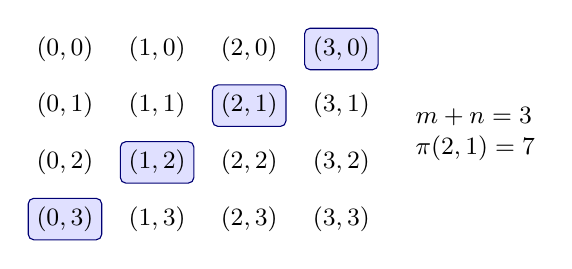
\begin{tikzpicture}[x=1.17cm,y=.72cm,font=\small]
  \foreach \m in {0,1,2,3}{
    \foreach \n in {0,1,2,3}{
      \node[inner sep=2pt] at (\m,-\n) {$(\m,\n)$};
    }
  }
  \foreach \m/\n in {0/3,1/2,2/1,3/0}{
    \node[rounded corners=2pt,fill=blue!12,draw=blue!45!black,
          inner sep=3pt] at (\m,-\n) {$(\m,\n)$};
  }
  \node[align=left,anchor=west] at (3.7,-1.5)
      {$m+n=3$\\$\pi(2,1)=7$};
\end{tikzpicture}
\caption{Fragment siatki $\N^2$: wyróżnione pary
z przekątnej $m+n=3$.}
\label{fig:card-pairing-diagonal}
\end{figure}

\begin{uwaga}[Gdzie pojawia się aksjomat wyboru?]
Dowód dla dwóch ustalonych zbiorów nie wymaga AC: dwie egzystencjalne przesłanki pozwalają wybrać dwa świadki bez postulatu jednoczesnego wyboru z nieskończonej rodziny. Natomiast zdanie „przeliczalna suma przeliczalnych zbiorów jest przeliczalna” może wymagać słabszej zasady wyboru: aby z przeliczalnej rodziny zbiorów przeliczalnych wybrać jednocześnie ich enumeracje. Wrócimy do tego w rozdziale o słabszych zasadach wyboru.
\end{uwaga}
\begin{twierdzenie}[Moc zbioru liczb rzeczywistych]\label{thm:card-continuum}
Istnieje bijekcja $\R\to\mathcal P(\N)$; zatem $\mathfrak c=2^{\aleph_0}>\aleph_0$.
\end{twierdzenie}
\begin{proof}
Najpierw skonstruujmy iniekcję $\mathcal P(\N)\to[0,1]$ przez
\[
S\longmapsto \sum_{n\in S}\frac{2}{3^{n+1}}.
\]
Dla dwóch różnych zbiorów niech $k$ będzie najmniejszym indeksem różnicy. Różnica wkładów na pozycji $k$ ma moduł $2/3^{k+1}$, a suma modułów wszystkich późniejszych wkładów wynosi $1/3^{k+1}$. Wartości są więc różne.

W drugą stronę każdej liczbie rzeczywistej $x$
przypiszmy jej przekrój
$D_x:=\{q\in\Q:q<x\}$.
Zbiór ten istnieje przez separację.
Jeśli $x<y$, to z gęstości $\Q$ w $\R$
istnieje $q\in\Q$ z $x<q<y$,
a więc $q\in D_y\setminus D_x$.
Stąd przyporządkowanie $x\mapsto D_x$
jest iniekcją $\R\to\mathcal P(\Q)$.

Zbudujmy teraz konkretną iniekcję $j:\Q\to\N$.
Każda liczba wymierna ma dokładnie jedno
przedstawienie $q=a/b$, gdzie $a\in\Z$,
$b\in\N\setminus\{0\}$ i $\gcd(|a|,b)=1$.
Zdefiniujmy iniekcję $\gamma:\Z\to\N$
przez $\gamma(a)=2a$ dla $a\ge0$
i $\gamma(a)=-2a-1$ dla $a<0$.
Następnie połóżmy
$j(q):=\pi(\gamma(a),b-1)$,
gdzie $\pi$ jest bijekcją
z Twierdzenia~\ref{thm:card-n2}.
Jednoznaczność zredukowanego ułamka,
iniektywność $\gamma$ i $\pi$
dowodzą iniektywności $j$.
Przyporządkowanie $S\mapsto j[S]$
jest zatem iniekcją
$\mathcal P(\Q)\to\mathcal P(\N)$,
bez potrzeby wyboru dowolnej enumeracji.

Złożyliśmy iniekcję
$\R\to\mathcal P(\Q)\to\mathcal P(\N)$.
W przeciwną stronę skonstruowaliśmy
iniekcję $\mathcal P(\N)\to[0,1]\subseteq\R$.
Twierdzenie~\ref{thm:card-cb} daje bijekcję
$\R\to\mathcal P(\N)$, zgodnie z tezą.
\end{proof}
\begin{uwaga}[Czego nie rozstrzyga twierdzenie Cantora?]
Wiemy, że $\aleph_0<\mathfrak c=2^{\aleph_0}$. Pytanie, czy istnieje moc ściśle pośrednia między $\aleph_0$ a $\mathfrak c$, to hipoteza continuum. Sam dowód diagonalny nie rozstrzyga tej hipotezy.
\end{uwaga}

\section{Dlaczego $\N$ i $\R$ nie są równoliczne?}\label{sec:card-n-vs-r}
\begin{twierdzenie}[Nieprzeliczalność prostej rzeczywistej]\label{thm:card-n-not-r}
Nie istnieje surjekcja $e:\N\to\R$.
W szczególności nie istnieje bijekcja $\N\to\R$, a ponieważ
funkcja $n\mapsto n$ jest iniekcją $\N\to\R$, zachodzi
\[
|\N|<|\R|.
\]
\end{twierdzenie}
\begin{proof}
\emph{Krok 1: zakodowanie podzbiorów liczb naturalnych liczbami rzeczywistymi.}
Dla $S\subseteq\N$ połóżmy
\[
 c(S):=\sum_{n=0}^{\infty}\frac{2\chi_S(n)}{3^{n+1}}\in[0,1],
\]
gdzie $\chi_S(n)=1$ dla $n\in S$ i $\chi_S(n)=0$ w przeciwnym przypadku.
Szereg jest zbieżny, ponieważ jego wyrazy są nieujemne i
$\sum_{n=0}^{\infty}2/3^{n+1}=1$.

Pokażemy, że $c$ jest iniekcją. Niech $S\ne T$ i niech $k$
będzie najmniejszą liczbą naturalną należącą do dokładnie
jednego z tych zbiorów. Przyjmijmy dla ustalenia uwagi, że
$k\in S\setminus T$. Wówczas składniki szeregu dla $n<k$ są identyczne,
a składnik dla $n=k$ jest w $c(S)$ większy o $2/3^{k+1}$.
Cała możliwa różnica późniejszych składników ma moduł
nie większy niż
\[
\sum_{n=k+1}^{\infty}\frac{2}{3^{n+1}}
=\frac{1}{3^{k+1}}.
\]
Stąd $c(S)-c(T)\ge 1/3^{k+1}>0$, więc $c(S)\ne c(T)$.

\emph{Krok 2: sprzeczność z domniemaną enumeracją liczb rzeczywistych.}
Załóżmy, że istnieje surjekcja $e:\N\to\R$.
Dla każdego $n\in\N$ określmy zbiór $S_n$ następująco:
jeśli $e(n)$ jest postaci $c(S)$ dla jakiegoś $S\subseteq\N$,
to $S_n$ oznacza ten \emph{jedyny} zbiór $S$;
w przeciwnym razie kładziemy $S_n=\varnothing$.
Jednoznaczność w pierwszym przypadku wynika z kroku pierwszego.
Nie dokonujemy tu żadnego nieuzasadnionego wyboru z wielu możliwości.

\emph{Krok 3: diagonalizacja.}
Zbudujmy zbiór
\[
D:=\{n\in\N:n\notin S_n\}.
\]
Jest to podzbiór $\N$. Liczba $c(D)$ jest rzeczywista,
a $e$ jest — z założenia — surjekcją, więc dla pewnego $k\in\N$
zachodzi $e(k)=c(D)$. Wtedy definicja $S_k$ daje $S_k=D$.
Sprawdzamy teraz, czy $k$ należy do $D$:
\[
 k\in D\quad\Longleftrightarrow\quad k\notin S_k
 \quad\Longleftrightarrow\quad k\notin D.
\]
Otrzymaliśmy sprzeczność. Dlatego surjekcja $\N\to\R$
nie istnieje, a zatem $\N$ i $\R$ nie są równoliczne.
\end{proof}
\begin{uwaga}[Dlaczego użyliśmy cyfr $0$ i $2$ w bazie trójkowej?]
Zwykłe rozwinięcia dziesiętne mają niejednoznaczności,
na przykład $0{,}999\ldots=1$. W powyższej konstrukcji
nie musimy zakładać jednoznaczności ogólnego rozwinięcia
trójkowego: oszacowanie pierwszego różniącego się składnika
samodzielnie dowodzi, że różnym zbiorom $S$ odpowiadają różne liczby.
To właśnie sprawdzenie zapobiega pominięciu istotnej trudności.
\end{uwaga}

\section{Jawne bijekcje między przedziałami a prostą}\label{sec:card-interval-bijections}
\begin{twierdzenie}[Otwarty przedział i prosta są równoliczne]\label{thm:card-open-interval-real}
Istnieje bijekcja $F:\R\to(0,1)$. Jedną z nich jest
\[
F(x):=\frac12\left(1+\frac{x}{1+|x|}\right).
\]
\end{twierdzenie}
\begin{proof}
\emph{Krok 1: sprawdzenie wartości.}
Dla każdego $x\in\R$ zachodzi $|x|<1+|x|$,
a więc $-1<x/(1+|x|)<1$. Dodając $1$ i dzieląc przez $2$,
otrzymujemy $0<F(x)<1$. Wzór rzeczywiście określa funkcję
$F:\R\to(0,1)$.

\emph{Krok 2: wyprowadzenie funkcji odwrotnej.}
Niech $t\in(0,1)$, a $u:=2t-1$. Wtedy $-1<u<1$, zatem
$1-|u|>0$. Połóżmy
\[
G(t):=\frac{2t-1}{1-|2t-1|}=\frac{u}{1-|u|}.
\]
Wzór jest dobrze określony dla każdego $t\in(0,1)$.
Wykażemy dwie równości, które oznaczają, że $F$ i $G$
są funkcjami wzajemnie odwrotnymi.

\emph{Krok 3: sprawdzenie $F(G(t))=t$.}
Dla $x=G(t)=u/(1-|u|)$ mamy
\[
1+|x|=1+\frac{|u|}{1-|u|}=\frac{1}{1-|u|},
\qquad \frac{x}{1+|x|}=u.
\]
Stąd $F(G(t))=(1+u)/2=t$.

\emph{Krok 4: sprawdzenie $G(F(x))=x$.}
Dla dowolnego $x\in\R$ połóżmy $u=x/(1+|x|)$.
Wtedy $2F(x)-1=u$ i
$1-|u|=1/(1+|x|)$. Zatem
\[
G(F(x))=\frac{u}{1-|u|}
=\frac{x/(1+|x|)}{1/(1+|x|)}=x.
\]
Dwie tożsamości dowodzą bijektywności $F$.
\end{proof}
\begin{przyklad}[Jak działa ta bijekcja?]
Dla $x=0$ otrzymujemy $F(0)=1/2$; dla $x=1$ mamy
$F(1)=3/4$, a dla $x=-1$ mamy $F(-1)=1/4$.
Gdy $x$ rośnie bez ograniczenia, wartości $F(x)$
zbliżają się do $1$ od dołu; gdy $x$ maleje bez ograniczenia,
zbliżają się do $0$ od góry. Żaden argument nie daje
wartości $0$ ani $1$, zgodnie z przeciwdziedziną $(0,1)$.
\end{przyklad}

\begin{twierdzenie}[Przedział otwarty i półotwarty są równoliczne]\label{thm:card-open-half-open}
Istnieje bijekcja $H:(0,1)\to(0,1]$, mimo że $(0,1)$
jest właściwym podzbiorem $(0,1]$.
\end{twierdzenie}
\begin{proof}
\emph{Krok 1: wskazanie punktów do przesunięcia.}
Rozważmy ciąg różnych elementów przedziału $(0,1)$:
\[
\frac12,\ \frac13,\ \frac14,\ \frac15,\ \ldots
\]
Chcemy przesunąć każdą z tych liczb na poprzednie miejsce,
a pierwszą z nich przenieść do punktu $1$, którego brakuje
w dziedzinie.

\emph{Krok 2: ścisła definicja funkcji.}
Dla $x\in(0,1)$ określmy
\[
H(x):=
\begin{cases}
\dfrac{1}{n-1},&\text{gdy }x=\dfrac1n\text{ dla }n\in\N,\ n\ge2,\\[3pt]
x,&\text{gdy }x\notin\{\dfrac1n:n\in\N,\ n\ge2\}.
\end{cases}
\]
Ponieważ liczby $1/n$ są parami różne, pierwszy przypadek
nigdy nie przypisuje temu samemu argumentowi różnych wartości.
Pierwszy przypadek daje element $(0,1]$ (dla $n=2$ jest to $1$),
a drugi daje element $(0,1)$. Funkcja jest dobrze określona.

\emph{Krok 3: zbudowanie odwrotności.}
Zdefiniujmy $K:(0,1]\to(0,1)$ przez
\[
K(y):=
\begin{cases}
\dfrac12,&\text{gdy }y=1,\\[3pt]
\dfrac{1}{n+1},&\text{gdy }y=\dfrac1n\text{ dla }n\in\N,\ n\ge2,\\[3pt]
y,&\text{gdy }y\notin\{1\}\cup\{\dfrac1n:n\in\N,\ n\ge2\}.
\end{cases}
\]
Trzy przypadki są rozłączne i obejmują wszystkie $y\in(0,1]$.
Dla $x=1/2$ mamy $K(H(x))=K(1)=1/2$.
Dla $x=1/n$, $n\ge3$, dostajemy
$K(H(1/n))=K(1/(n-1))=1/n$.
Jeśli $x$ nie jest żadnym $1/n$, obie funkcje pozostawiają go bez zmian.
Zatem $K\circ H=\operatorname{id}_{(0,1)}$.

W drugą stronę: $H(K(1))=H(1/2)=1$;
dla $y=1/n$, $n\ge2$, zachodzi
$H(K(y))=H(1/(n+1))=1/n=y$;
pozostałe wartości również pozostają bez zmian.
Stąd $H\circ K=\operatorname{id}_{(0,1]}$.
Otrzymaliśmy funkcje wzajemnie odwrotne, więc $H$ jest bijekcją.
\end{proof}
\begin{przyklad}[Co dzieje się z konkretnymi punktami?]
$H(1/2)=1$, $H(1/3)=1/2$, $H(1/4)=1/3$,
natomiast $H(2/3)=2/3$.
Wszystkie punkty poza przeliczalnym ciągiem $1/2,1/3,\ldots$
pozostają na swoich miejscach. Jednocześnie żaden punkt nie ginie:
na miejsce $1/2$ trafia $1/3$, na miejsce $1/3$ trafia $1/4$
i tak dalej. Na tym polega „zrobienie miejsca” dla nowego punktu $1$.
\end{przyklad}

\begin{wniosek}[Trzy zbiory tej samej mocy]\label{cor:card-interval-real}
Zachodzi $(0,1)\approx(0,1]\approx\R$.
W szczególności $|(0,1)|=|(0,1]|=|\R|$.
\end{wniosek}
\begin{proof}
Twierdzenie~\ref{thm:card-open-interval-real} daje bijekcję
$F:\R\to(0,1)$, a Twierdzenie~\ref{thm:card-open-half-open}
daje bijekcję $H:(0,1)\to(0,1]$.
Złożenie $H\circ F:\R\to(0,1]$ jest bijekcją,
ponieważ ma funkcję odwrotną $F^{-1}\circ H^{-1}$.
Jest to wniosek z definicji równoliczności, bez stosowania
jakiegokolwiek dodatkowego aksjomatu wyboru.
\end{proof}
\begin{uwaga}[Nie mylmy liczności z długością przedziału]
Zbiory $(0,1)$, $(0,1]$ i $\R$ mają tę samą \emph{moc},
ale nie tę samą długość. Równoliczność wymaga bijekcji,
nie zaś zachowania odległości, długości czy ciągłości.
Funkcja $H$ nie jest ciągła w punktach $1/n$, lecz
ciągłość nie występuje w definicji równoliczności.
\end{uwaga}

\section{Rozróżnienie wyboru i porównywalności mocy}
\begin{twierdzenie}[Porównywalność mocy a aksjomat wyboru]
\label{thm:card-comparability-choice}
W teorii ZF następujące warunki są równoważne:
\begin{enumerate}[label=(\roman*)]
\item obowiązuje aksjomat wyboru;
\item dla dowolnych zbiorów $A,B$ istnieje
iniekcja $A\to B$ albo iniekcja $B\to A$.
\end{enumerate}
\end{twierdzenie}
\begin{proof}
Załóżmy AC. Z Twierdzenia~\ref{thm:choice-wellorder}
każdy z dwóch ustalonych zbiorów $A,B$
ma dobry porządek. Lemat o porównywaniu dobrych
porządków (Lemat~\ref{lem:choice-wellorder-comparison})
daje izomorfizm jednego z nich z całym drugim
lub z jego właściwym odcinkiem początkowym.
Złożenie z włączeniem odcinka początkowego
do całego zbioru daje wymaganą iniekcję.
Dwa ustalone dobre porządki można wskazać
bez dodatkowej zasady wyboru.

Odwrotnie, załóżmy porównywalność wszystkich
zbiorów i ustalmy dowolny zbiór $A$.
Twierdzenie Hartogsa~\ref{thm:choice-hartogs}
daje dobrze uporządkowany zbiór $H(A)$,
dla którego nie istnieje iniekcja $H(A)\to A$.
Z porównywalności wynika więc iniekcja
$j:A\to H(A)$. Przenieśmy porządek z $H(A)$
na $A$ przez
$a\prec b$ wtedy i tylko wtedy, gdy
$j(a)<_{H(A)}j(b)$.
Dla każdego niepustego $X\subseteq A$
jego obraz $j[X]$ ma element najmniejszy;
ponieważ $j$ jest iniekcją, element ten ma
dokładnie jeden przeciwobraz w $X$, który
jest najmniejszym elementem $X$.
Zatem $\prec$ jest dobrym porządkiem na $A$.
Ponieważ $A$ był dowolny, obowiązuje zasada
dobrego uporządkowania, a z
Twierdzenia~\ref{thm:choice-equivalence}
wynika AC.
\end{proof}
\begin{uwaga}[Unikanie błędnego koła]
\label{rem:card-no-circular-choice}
Używany tutaj zbiór $H(A)$ skonstruowano w ZF
w rozdziale~\ref{ch:axiom-choice}, bez
liczb porządkowych i bez aksjomatu wyboru.
Dopiero w rozdziale~\ref{ch:ordinals}
zdefiniujemy ordynały i opiszemy je
jako kanoniczne reprezentacje dobrych porządków.
Samo twierdzenie Cantora--Bernsteina
nie zapewnia porównywalności wszystkich mocy.
\end{uwaga}
